\documentclass{beamer}
\usepackage{ragged2e}
\usepackage{CJKutf8}
\usepackage{tikz}
\setbeamertemplate{theorems}[numbered]
\justifying\let\raggedright\justifying
\begin{document}
\begin{CJK*}{UTF8}{gbsn}

  \newtheorem{Thm}{定理}
  \newtheorem{Thm1}{定理}

\theoremstyle{definition}
\newtheorem{Def}{定义}
\theoremstyle{example}
\newtheorem*{Ex}{例:}
\newtheorem*{Exercise}{习题}
\newtheorem{Exercise1}{习题}

\date{}
\author{陈建文}
\title{习题讲解}
\begin{frame}
  \titlepage
\end{frame}



  \begin{frame}
    具有$4$个顶点的互相不同构的所有无向图:

    \vspace{0.3cm}
  \centering
  \begin{minipage}{0.24\linewidth}
    \centering
    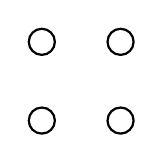
\begin{tikzpicture}[auto,
    specification/.style ={circle, draw, thick}]
   \node[specification] (A) at (0,0)  {};
   \node[specification] (B)  at (0,1)  {};
   \node[specification] (C)  at (1,1)  {};
   \node[specification] (D) at (1,0)  {};
 \end{tikzpicture}\\
 \vspace*{0.3cm}
 A
\end{minipage}\hfill 
  \begin{minipage}{0.24\linewidth}
    \centering
    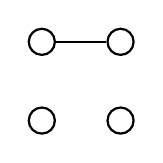
\begin{tikzpicture}[auto,
    specification/.style ={circle, draw, thick}]
   \node[specification] (A) at (0,0)  {};
   \node[specification] (B) at (0,1)  {};
   \node[specification] (C) at (1,1)  {};
   \node[specification] (D) at (1,0)  {};
   \draw[thick] (B) to  (C);
 \end{tikzpicture}\\
 \vspace*{0.3cm}
 B
\end{minipage}\hfill 
  \begin{minipage}{0.24\linewidth}
    \centering
    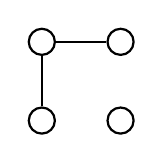
\begin{tikzpicture}[auto,
    specification/.style ={circle, draw, thick}]
   \node[specification] (A) at (0,0)  {};
   \node[specification] (B) at (0,1)  {};
   \node[specification] (C) at (1,1)  {};
   \node[specification] (D) at (1,0)  {};
   \draw[thick] (A) to  (B);
   \draw[thick] (B) to  (C);
 \end{tikzpicture}\\
 \vspace*{0.3cm}
 C
\end{minipage}\hfill 
  \begin{minipage}{0.24\linewidth}
    \centering
    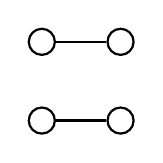
\begin{tikzpicture}[auto,
    specification/.style ={circle, draw, thick}]
   \node[specification] (A)  at (0,0)  {};
   \node[specification] (B)  at (0,1)  {};
   \node[specification] (C)  at (1,1)  {};
   \node[specification] (D) at (1,0)  {};
   \draw[thick] (B) to  (C);
   \draw[thick] (D) to  (A);
 \end{tikzpicture}\\
 \vspace*{0.3cm}
 D
\end{minipage}\hfill

\vspace*{0.5cm}
  \begin{minipage}{0.24\linewidth}
    \centering
    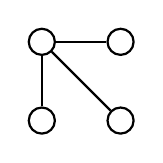
\begin{tikzpicture}[auto,
    specification/.style ={circle, draw, thick}]
   \node[specification] (A) at (0,0)  {};
   \node[specification] (B)  at (0,1)  {};
   \node[specification] (C)  at (1,1)  {};
   \node[specification] (D) at (1,0)  {};
   \draw[thick] (A) to (B);
   \draw[thick] (B) to (C);
      \draw[thick] (B) to (D);
 \end{tikzpicture}\\
 \vspace*{0.3cm}
 E
\end{minipage}\hfill
  \begin{minipage}{0.24\linewidth}
    \centering
    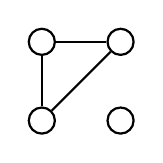
\begin{tikzpicture}[auto,
    specification/.style ={circle, draw, thick}]
   \node[specification] (A) at (0,0)  {};
   \node[specification] (B) at (0,1)  {};
   \node[specification] (C) at (1,1)  {};
   \node[specification] (D) at (1,0)  {};
   \draw[thick] (A) to  (B);
   \draw[thick] (B) to (C);
      \draw[thick] (C) to (A);
 \end{tikzpicture}\\
 \vspace*{0.3cm}
 F
\end{minipage}\hfill
  \begin{minipage}{0.24\linewidth}
    \centering
    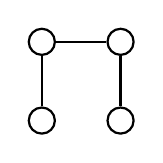
\begin{tikzpicture}[auto,
    specification/.style ={circle, draw, thick}]
   \node[specification] (A) at (0,0)  {};
   \node[specification] (B) at (0,1)  {};
   \node[specification] (C) at (1,1)  {};
   \node[specification] (D) at (1,0)  {};
   \draw[thick] (A) to  (B);
   \draw[thick] (B) to  (C);
      \draw[thick] (C) to (D);
 \end{tikzpicture}\\
 \vspace*{0.3cm}
 G
\end{minipage}\hfill 
  \begin{minipage}{0.24\linewidth}
    \centering
    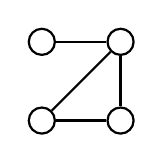
\begin{tikzpicture}[auto,
    specification/.style ={circle, draw, thick}]
   \node[specification] (A)  at (0,0)  {};
   \node[specification] (B)  at (0,1)  {};
   \node[specification] (C)  at (1,1)  {};
   \node[specification] (D) at (1,0)  {};
   \draw[thick] (A) to  (C);
   \draw[thick] (C) to  (D);
   \draw[thick] (D) to (A);
   \draw[thick] (C) to (B);
 \end{tikzpicture}\\
 \vspace*{0.3cm}
 H
\end{minipage}\hfill 

\vspace*{0.5cm}
\flushleft
  \begin{minipage}{0.24\linewidth}
    \centering
    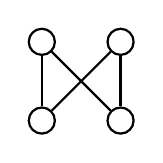
\begin{tikzpicture}[auto,
    specification/.style ={circle, draw, thick}]
   \node[specification] (A) at (0,0)  {};
   \node[specification] (B)  at (0,1)  {};
   \node[specification] (C)  at (1,1)  {};
   \node[specification] (D) at (1,0)  {};
   \draw[thick] (A) to (B);
   \draw[thick] (B) to (D);
   \draw[thick] (D) to (C);
      \draw[thick] (C) to (A);
 \end{tikzpicture}\\
 \vspace*{0.3cm}
 I
\end{minipage}
  \begin{minipage}{0.24\linewidth}
    \centering
    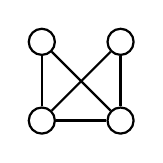
\begin{tikzpicture}[auto,
    specification/.style ={circle, draw, thick}]
   \node[specification] (A) at (0,0)  {};
   \node[specification] (B) at (0,1)  {};
   \node[specification] (C) at (1,1)  {};
   \node[specification] (D) at (1,0)  {};
   \draw[thick] (A) to  (B);
      \draw[thick] (C) to (D);
   \draw[thick] (D) to (A);
   \draw[thick] (A) to (C);
   \draw[thick] (B) to (D);
 \end{tikzpicture}\\
 \vspace*{0.3cm}
 J
\end{minipage} 
  \begin{minipage}{0.24\linewidth}
    \centering
    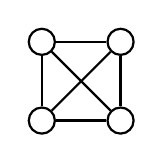
\begin{tikzpicture}[auto,
    specification/.style ={circle, draw, thick}]
   \node[specification] (A) at (0,0)  {};
   \node[specification] (B) at (0,1)  {};
   \node[specification] (C) at (1,1)  {};
   \node[specification] (D) at (1,0)  {};
   \draw[thick] (A) to  (B);
   \draw[thick] (B) to  (C);
      \draw[thick] (C) to (D);
   \draw[thick] (D) to (A);
   \draw[thick] (A) to (C);
   \draw[thick] (B) to (D);
 \end{tikzpicture}\\
 \vspace*{0.3cm}
 K
\end{minipage}
\end{frame}

\begin{frame}
  \begin{minipage}{0.24\linewidth}
    \centering
    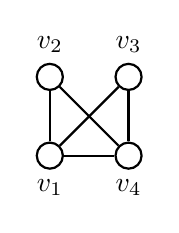
\begin{tikzpicture}[auto,
    specification/.style ={circle, draw, thick}]
   \node[specification] (A) [label=270:$v_1$] at (0,0)  {};
   \node[specification] (B) [label=90:$v_2$] at (0,1)  {};
   \node[specification] (C) [label=90:$v_3$] at (1,1)  {};
   \node[specification] (D) [label=270: $v_4$] at (1,0)  {};
   \draw[thick] (A) to  (B);
      \draw[thick] (C) to (D);
   \draw[thick] (D) to (A);
   \draw[thick] (A) to (C);
   \draw[thick] (B) to (D);
 \end{tikzpicture}\\
 \vspace*{0.3cm}
 J
\end{minipage}
\begin{minipage}{0.75\linewidth}
  \begin{equation*}
    \begin{split}
  J&=(V,E)\\
  V&=\{v_1,v_2,v_3,v_4\}\\
  E&=\{\{v_1,v_2\},\{v_1,v_3\},\{v_1,v_4\},\{v_2,v_4\},\{v_3,v_4\}\}
    \end{split}
  \end{equation*}
\end{minipage}
\end{frame}
\begin{frame}
    \begin{Def}\justifying\let\raggedright\justifying
  设$G=(V,E)$为一个图,$V=\{v_1,v_2,\ldots,v_p\}$。\\ $p\times p$矩阵$A=(a_{ij})$称为$G$的邻接矩阵,其中
  \[a_{ij}=\begin{cases}
      1, \text{如果}\{v_i,v_j\}\in E\\
      0, \text{如果}\{v_i,v_j\}\notin E\\
    \end{cases}
  \]
\end{Def}
  \begin{minipage}{0.3\linewidth}
    \centering
    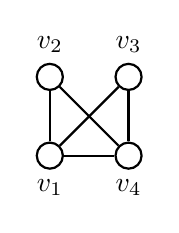
\begin{tikzpicture}[auto,
    specification/.style ={circle, draw, thick}]
   \node[specification] (A) [label=270:$v_1$] at (0,0)  {};
   \node[specification] (B) [label=90:$v_2$] at (0,1)  {};
   \node[specification] (C) [label=90:$v_3$] at (1,1)  {};
   \node[specification] (D) [label=270: $v_4$] at (1,0)  {};
   \draw[thick] (A) to  (B);
      \draw[thick] (C) to (D);
   \draw[thick] (D) to (A);
   \draw[thick] (A) to (C);
   \draw[thick] (B) to (D);
 \end{tikzpicture}\\
 \vspace*{0.3cm}
 J
\end{minipage}
\begin{minipage}{0.5\linewidth}
\begin{equation*}
  A=\begin{bmatrix}
    0&1&1&1\\
    1&0&0&1\\
    1&0&0&1\\
    1&1&1&0
  \end{bmatrix}
\end{equation*}
\end{minipage}
\end{frame}

\begin{frame}
    \begin{minipage}{0.24\linewidth}
    \centering
      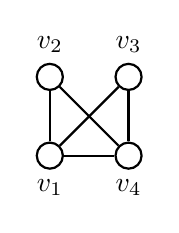
\begin{tikzpicture}[auto,
    specification/.style ={circle, draw, thick}]
   \node[specification] (A) [label=270:$v_1$] at (0,0)  {};
   \node[specification] (B) [label=90:$v_2$] at (0,1)  {};
   \node[specification] (C) [label=90:$v_3$] at (1,1)  {};
   \node[specification] (D) [label=270: $v_4$] at (1,0)  {};
   \draw[thick] (A) to  (B);
      \draw[thick] (C) to (D);
   \draw[thick] (D) to (A);
   \draw[thick] (A) to (C);
   \draw[thick] (B) to (D);
 \end{tikzpicture}\\
 \vspace*{0.3cm}
 J
\end{minipage}
\begin{minipage}{0.75\linewidth}
  顶点$v_1$和$v_4$之间有多少条不同的长度为$3$的通道?\pause
    \begin{Def}
    设$G=(V,E)$为一个图。$G$的一条通道是$G$的顶点和边的一个交错序列
    \[v_0,x_1,v_1,x_2,v_2,x_3,\ldots,v_{n-1},x_n,v_n\]
    其中$x_i=v_{i-1}v_i,i=1,2,\ldots,n$。$n$称为通道的长。这样的通道常称为$v_0-v_n$通道,并简记为$v_0v_1v_2\ldots   v_n$。
  \end{Def}\pause
  顶点$v_1$和$v_4$之间有$5$条不同的长度为$3$的通道:

  $v_1v_2v_1v_4$, $v_1v_3v_1v_4$, $v_1v_4v_1v_4$, $v_1v_4v_2v_4$, $v_1v_4v_3v_4$。
\end{minipage}
\end{frame}
\begin{frame}
    \begin{minipage}{0.24\linewidth}
    \centering
      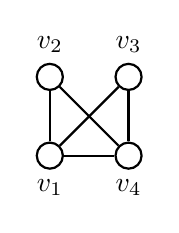
\begin{tikzpicture}[auto,
    specification/.style ={circle, draw, thick}]
   \node[specification] (A) [label=270:$v_1$] at (0,0)  {};
   \node[specification] (B) [label=90:$v_2$] at (0,1)  {};
   \node[specification] (C) [label=90:$v_3$] at (1,1)  {};
   \node[specification] (D) [label=270: $v_4$] at (1,0)  {};
   \draw[thick] (A) to  (B);
      \draw[thick] (C) to (D);
   \draw[thick] (D) to (A);
   \draw[thick] (A) to (C);
   \draw[thick] (B) to (D);
 \end{tikzpicture}\\
 \vspace*{0.3cm}
 J
\end{minipage}
\begin{minipage}{0.75\linewidth}
  顶点$v_1$和$v_4$之间有多少条不同的长度为$3$通道?
  \begin{equation*}
    A^3_{14} = A^2_{11}A_{14} + A^2_{12}A_{24} + A^2_{13}A_{34} + A^2_{14}A_{44}
  \end{equation*}
  其中
  \begin{align*}
    A^2_{11}&=A_{11}A_{11} + A_{12}A_{21} + A_{13}A_{31} + A_{14}A_{41}=3\\
    A^2_{12}&=A_{11}A_{12} + A_{12}A_{22} + A_{13}A_{32} + A_{14}A_{42}=1\\
    A^2_{13}&=A_{11}A_{13} + A_{12}A_{23} + A_{13}A_{33} + A_{14}A_{43}=1\\
    A^2_{14}&=A_{11}A_{14} + A_{12}A_{24} + A_{13}A_{34} + A_{14}A_{44}=2\\
    P^2_{11}&=\{v_1v_2v_1,v_1v_3v_1,v_1v_4v_1\}\\
    P^2_{12}&=\{v_1v_4v_2\}\\
    P^2_{13}&=\{v_1v_4v_3\}\\
    P^3_{14}&=\{v_1v_2v_1v_4,v_1v_3v_1v_4,v_1v_4v_1v_4,v_1v_4v_2v_4,v_1v_4v_3v_4\}
  \end{align*}
\end{minipage}
\end{frame}

\begin{frame}
    \begin{Thm}
    设$G=(V,E)$为一个(p,q)图,$p\times p$矩阵$A$为$G$的邻接矩阵,则$G$中$v_i$与
    $v_j$间长为$l$的通道的条数等于$A^l$的第$i$行第$j$列元素的值。
  \end{Thm}
  \begin{proof}[证明]
      用数学归纳法证明,施归纳于$l$。

  当$l=1$时,结论显然成立。

  假设当$l=k$时结论成立,往证当$l=k+1$时结论也成立。由矩阵乘法的计算规则知:
  \[(A^{k+1})_{ij} = (A^{k}A)_{ij} = \sum_{h=1}^p(A^k)_{ih}A_{hj}\]

  由归纳假设,$(A^k)_{ih}$为从顶点$v_i$到顶点$v_h$长度为$k$的通道的条数。

  由从顶点$v_i$到顶点$v_j$长度为$k+1$的通道的条数为从顶点$v_i$到顶点$v_j$长度为
  $k+1$且倒数第二个顶点依次为$v_1$,$v_2$,$\ldots$,$v_p$的通道的条数之和
  知$(A^{k+1})_{ij}$为从顶点$v_i$到顶点$v_j$长度为$k+1$的通道的条数。
  \end{proof}
\end{frame}

\begin{frame}
  \begin{minipage}{0.3\linewidth}
    \centering
    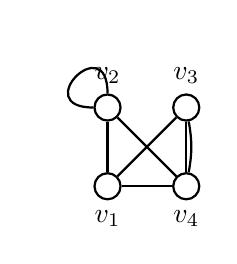
\begin{tikzpicture}[auto,
    specification/.style ={circle, draw, thick}]
   \node[specification] (A) [label=270:$v_1$] at (0,0)  {};
   \node[specification] (B) [label=90:$v_2$] at (0,1)  {};
   \node[specification] (C) [label=90:$v_3$] at (1,1)  {};
   \node[specification] (D) [label=270: $v_4$] at (1,0)  {};
   \draw[thick] (A) to  (B);
      \draw[thick] (C) to (D);
   \draw[thick] (D) to (A);
   \draw[thick] (A) to (C);
   \draw[thick] (B) to (D);
   \draw[thick] (C) to [bend left = 10] (D);
   \draw[thick] (B) ..controls +(up:10mm) and +(left:10mm) .. (B);
 \end{tikzpicture}\\
 \vspace*{0.3cm}
 J
\end{minipage}
\begin{minipage}{0.7\linewidth}
\begin{equation*}
  A=\begin{bmatrix}
    0&1&1&1\\
    1&1&0&1\\
    1&0&0&2\\
    1&1&2&0
  \end{bmatrix}
\end{equation*}  
\end{minipage}
    \begin{Def}\justifying\let\raggedright\justifying
  设$G=(V,E)$为一个图,$V=\{v_1,v_2,\ldots,v_p\}$。\\ $p\times p$矩阵$A=(a_{ij})$称为$G$的邻接矩阵,其中
  $a_{ij}=$联结顶点$v_i$和$v_j$的边的条数。
\end{Def}
  
\end{frame}
\begin{frame}
  \begin{minipage}{0.25\linewidth}
    \centering
    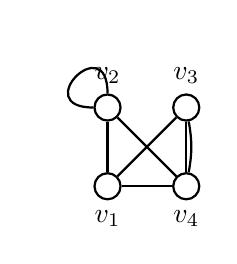
\begin{tikzpicture}[auto,
    specification/.style ={circle, draw, thick}]
   \node[specification] (A) [label=270:$v_1$] at (0,0)  {};
   \node[specification] (B) [label=90:$v_2$] at (0,1)  {};
   \node[specification] (C) [label=90:$v_3$] at (1,1)  {};
   \node[specification] (D) [label=270: $v_4$] at (1,0)  {};
   \draw[thick] (A) to  (B);
      \draw[thick] (C) to (D);
   \draw[thick] (D) to (A);
   \draw[thick] (A) to (C);
   \draw[thick] (B) to (D);
   \draw[thick] (C) to [bend left = 10] (D);
   \draw[thick] (B) ..controls +(up:10mm) and +(left:10mm) .. (B);
 \end{tikzpicture}\\
 \vspace*{0.3cm}
 J
\end{minipage}
\begin{minipage}{0.75\linewidth}
    \begin{Def}\justifying\let\raggedright\justifying
    设$G$为一个伪图。$G$的一条通道为$G$的顶点和边的一个交错序列
    \[v_0,x_1,v_1,x_2,v_2,x_3,\ldots,v_{n-1},x_n,v_n\]
    其中$x_i$为联结顶点$v_{i-1}$和顶点$v_{i}$的边,$i=1,2,\ldots,n$。$n$称为通道的长。这样的通道常称为$v_0-v_n$通道。当$v_0=v_n$时,则称此通道为闭通道。
  \end{Def}
  \begin{Def}
   如果伪图中一条通道上的各边互不相同,则称此通道为伪图的迹。如果一条闭通道上的各边互不相同,则此闭通道称为闭迹。
  \end{Def}
  \begin{Def}
    如果一条通道上的各顶点互不相同,则称此通道为路。如果闭通道上除终点外各顶点互不相同,则称此闭通道为圈,或回路。
  \end{Def}
\end{minipage}
\end{frame}
\begin{frame}
  \begin{minipage}{0.25\linewidth}
    \centering
    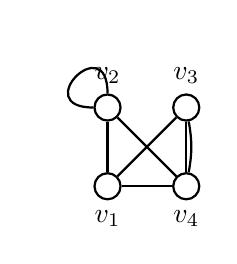
\begin{tikzpicture}[auto,
    specification/.style ={circle, draw, thick}]
   \node[specification] (A) [label=270:$v_1$] at (0,0)  {};
   \node[specification] (B) [label=90:$v_2$] at (0,1)  {};
   \node[specification] (C) [label=90:$v_3$] at (1,1)  {};
   \node[specification] (D) [label=270: $v_4$] at (1,0)  {};
   \draw[thick] (A) to  (B);
      \draw[thick] (C) to (D);
   \draw[thick] (D) to (A);
   \draw[thick] (A) to (C);
   \draw[thick] (B) to (D);
   \draw[thick] (C) to [bend left = 10] (D);
   \draw[thick] (B) ..controls +(up:10mm) and +(left:10mm) .. (B);
 \end{tikzpicture}\\
 \vspace*{0.3cm}
 J
\end{minipage}
\begin{minipage}{0.75\linewidth}
    \begin{Def}
   设$G$为一个伪图,如果$G$中任意两个不同顶点间至少有一条路联结,则称$G$为一个连通图。
 \end{Def}
\end{minipage}
\end{frame}

\begin{frame}
    \begin{Thm1}
    设$G=(V,E)$为一个(p,q)图,$p\times p$矩阵$A$为$G$的邻接矩阵,则$G$中$v_i$与
    $v_j$间长为$l$的通道的条数等于$A^l$的第$i$行第$j$列元素的值。
  \end{Thm1}
  \begin{proof}[证明]
      用数学归纳法证明,施归纳于$l$。

  当$l=1$时,结论显然成立。

  假设当$l=k$时结论成立,往证当$l=k+1$时结论也成立。由矩阵乘法的计算规则知:
  \[(A^{k+1})_{ij} = (A^{k}A)_{ij} = \sum_{h=1}^p(A^k)_{ih}A_{hj}\]

  由归纳假设,$(A^k)_{ih}$为从顶点$v_i$到顶点$v_h$长度为$k$的通道的条数。

  由从顶点$v_i$到顶点$v_j$长度为$k+1$的通道的条数为从顶点$v_i$到顶点$v_j$长度为
  $k+1$且倒数第二个顶点依次为$v_1$,$v_2$,$\ldots$,$v_p$的通道的条数之和
  知$(A^{k+1})_{ij}$为从顶点$v_i$到顶点$v_j$长度为$k+1$的通道的条数。
  \end{proof}
\end{frame}

\begin{frame}
\begin{Thm}
  设$G$为一个有$p$个顶点的连通图,$A$为它的邻接矩阵,则$G$为连通的当且仅当$(A+I)^{p-1}>0$。
\end{Thm}
\begin{proof}[证明]
  $\Rightarrow$ 设$G$为连通的,则对$G$的任意两个不同的顶点$v_i$与$v_j$间必有一条路。因此,存在$l$,$1\leq l \leq p-1$,$(A^l)_{ij}>0$。所以
  $\sum_{l=0}^{p-1}(A^l)_{ij}>0$。
  因此,\[(A+I)^{p-1}=I + C_{p-1}^{1}A + C_{p-1}^{2}A^2 + \cdots + A^{p-1} \geq \sum_{l=0}^{p-1}A^l > 0\]

  $\Leftarrow$ 设$(A+I)^{p-1}>0$。由于
  \[(A+I)^{p-1}=I + C_{p-1}^{1}A + C_{p-1}^{2}A^2 + \cdots + A^{p-1}  > 0\]
  所以,对任意的$i,j$,$1\leq i,j \leq p$,如果$i\neq j$,则存在$l$,$1\leq l \leq p-1$,使得$(A^l)_{ij}>0$。因此,$v_i$与$v_j$之间有长为$l$的通道,从而必有路。所以$G$为连通的。
\end{proof}
\end{frame}
\begin{frame}
  \begin{Thm1}
      设$G$为一个有$p$个顶点的连通图,$A$为它的邻接矩阵,则$G$为连通的当且仅当$(A+I)^{p-1}>0$。
    \end{Thm1}
  \begin{minipage}{0.2\linewidth}
    \centering
    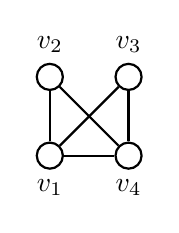
\begin{tikzpicture}[auto,
    specification/.style ={circle, draw, thick}]
   \node[specification] (A) [label=270:$v_1$] at (0,0)  {};
   \node[specification] (B) [label=90:$v_2$] at (0,1)  {};
   \node[specification] (C) [label=90:$v_3$] at (1,1)  {};
   \node[specification] (D) [label=270: $v_4$] at (1,0)  {};
   \draw[thick] (A) to  (B);
      \draw[thick] (C) to (D);
   \draw[thick] (D) to (A);
   \draw[thick] (A) to (C);
   \draw[thick] (B) to (D);
 \end{tikzpicture}\\
 \vspace*{0.3cm}
 G
\end{minipage}
  \begin{minipage}{0.2\linewidth}
    \centering
    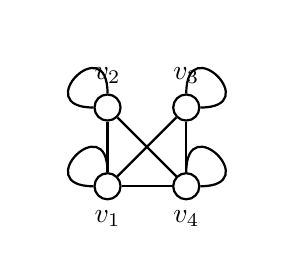
\begin{tikzpicture}[auto,
    specification/.style ={circle, draw, thick}]
   \node[specification] (A) [label=270:$v_1$] at (0,0)  {};
   \node[specification] (B) [label=90:$v_2$] at (0,1)  {};
   \node[specification] (C) [label=90:$v_3$] at (1,1)  {};
   \node[specification] (D) [label=270: $v_4$] at (1,0)  {};
   \draw[thick] (A) to  (B);
      \draw[thick] (C) to (D);
   \draw[thick] (D) to (A);
   \draw[thick] (A) to (C);
   \draw[thick] (B) to (D);
      \draw[thick] (A) ..controls +(up:10mm) and +(left:10mm) .. (A);
      \draw[thick] (B) ..controls +(up:10mm) and +(left:10mm) .. (B);
         \draw[thick] (C) ..controls +(up:10mm) and +(right:10mm) .. (C);
   \draw[thick] (D) ..controls +(up:10mm) and +(right:10mm) .. (D);
 \end{tikzpicture}\\
 \vspace*{0.3cm}
 G'
\end{minipage}\hfill
\begin{minipage}{0.5\linewidth}
\begin{proof}[证明]\justifying\let\raggedright\justifying
  设$G$为一个包含$p$个顶点的图,在$G$的每个顶点上添加一个环,得到一个带环图$G'$,则$G$为连通的当且仅当$G'$为连通的。$G'$为连通的,当且仅当对$G'$的任意两个不同的顶点$v_i$与$v_j$之间有路。在$G'$中$v_i$与$v_j$之间有路当且仅当$v_j$与$v_j$之间有长为$p-1$的通道,因此$G'$为连通的当且仅当$(A+I)^{p-1}>0$。从而$G$为连通的,当且仅当$(A+I)^{p-1}>0$。
\end{proof}  
\end{minipage}
  \end{frame}
\end{CJK*}
\end{document}
